% This is samplepaper.tex, a sample chapter demonstrating the
% LLNCS macro package for Springer Computer Science proceedings;
% Version 2.20 of 2017/10/04
%
\documentclass[runningheads]{llncs}
%
\usepackage{graphicx}


% Package to generate and customize Algorithm as per ACM style
\usepackage[ruled, linesnumbered, noend]{algorithm2e}
\renewcommand{\algorithmcfname}{Algorithm}
\SetAlFnt{\small}
\SetAlCapFnt{\small}
\SetAlCapNameFnt{\small}
\SetAlCapHSkip{0pt}
\IncMargin{-\parindent}
% Used for displaying a sample figure. If possible, figure files should
% be included in EPS format.
%
% If you use the hyperref package, please uncomment the following line
% to display URLs in blue roman font according to Springer's eBook style:
% \renewcommand\UrlFont{\color{blue}\rmfamily}

\newtheorem{defn}{Definition}

\begin{document}
%
\title{On the Valiant's Algorithm Parallelization\thanks{The research was supported by the Russian Science Foundation, grant No. 18-11-00100.}}
%
%\titlerunning{Abbreviated paper title}
% If the paper title is too long for the running head, you can set
% an abbreviated paper title here
%
\author{Yuliya Susanina\inst{1, 2} \and
Anna Yaveyn\inst{3} \and
Semyon Grigorev\inst{1, 2}\orcidID{0000-0002-7966-0698}}
%
\authorrunning{Yuliya Susanina, Anna Yaveyn, and Semyon Grigorev}
% First names are abbreviated in the running head.
% If there are more than two authors, 'et al.' is used.
%
\institute{Saint Petersburg State University, 7/9 Universitetskaya nab.\\ St. Petersburg, 199034 Russia \\
\and JetBrains Research, Universitetskaya emb., 7-9-11/5A \\ St.Petersburg, Russia \\
\email{jsusanina@gmail.com},
\email{semen.grigorev@jetbrains.com}\\
\and
...\\
\email{...}}
%
\maketitle              % typeset the header of the contribution
%
\begin{abstract}
Recent  research  has  shown  that the theory of formal languages can be used in bioinformatics. While using parsing for processing nucleotide sequences it became necessary to find an easily adaptable to the string-matching problem parsing algorithm, and as such field of application as bioinformatics requires working with large amount of data, it should be highly efficient. The asymptotically fastest parsing algorithm was proposed by Valiant and based on matrix multiplication. The original version of matrix-based algorithm is difficult to apply to the string-matching problem. In this paper we present  a modification  of Valiant's  algorithm dealing with the problem mentioned above. The modification has a succinct proof of correctness and is implemented.

\keywords{Parsing \and Matrix multiplication \and Context-free grammars.}
\end{abstract}
%
%
%
\section{Introduction}

Foundation in some areas: graphs, code analysis, etc.
Why is it important to proof B-H in Coq?
Bar-Hillel theorem is a main on �.
Short overview of current results.

\section{Background}

In this section we briefly introduce the key definitions and the necessary parsing algorithm.
Before descibing the Valiant's  algorithm, we would like to mention one of the basic recognition algorithms known as CYK (the Cocke-Younger-Kasami algorithm), by which we show the main Valiant's idea that made such time complexity possible.

\subsection{Preliminaries}

An alphabet $\Sigma$ is a finite nonempty set of symbols. $\Sigma^{*}$ is a set of all finite strings over $\Sigma$.
A grammar is a quadruple $(\Sigma, N, R, S)$, where $\Sigma$ is a finite set of terminals, $N$ is a finite set of nonterminals, $R$ is a finite set of productions of the form $\alpha \rightarrow \gamma$, where $\alpha \in V^{*}NV^{*}$, $\gamma \in V^{*}$, $V = \Sigma \cup N$ and $S \in N$ is a start symbol.

\begin{defn} Grammar $G = (\Sigma, N, R, S)$ is called context-free, if $\space\forall r \in R$ are of the form $A \rightarrow \beta$, where $A \in N, \beta \in V^{+}$.
\end{defn}

\begin{defn} Context-free grammar $G = (\Sigma, N, R, S)$ is said to be in Chomsky normal form if all productions in R are of the form:
\begin{itemize}
  \item $A \rightarrow BC$,
  \item $A \rightarrow a$,
  \item $S \rightarrow \varepsilon$,
\end{itemize}
where $A, B, C \in N, a \in \Sigma, \varepsilon$ is an empty string.
\end{defn}

\begin{defn} $L_{G}(A)$ is language of grammar $G_{A} = (\Sigma, N, R, A)$, which means all the sentences that can be derived in a finite number of rules applications from the start symbol $A$.
\end{defn}


\subsection{Parsing by matrix multiplication}

The main problem of parsing is to verify if the input string belongs to the language of some given grammar $G$. We will describe the Cocke-Younger-Kasami algorithm and the most asymptotically efficient parsing algorithm, which works for all context-free grammars, Valiant's parsing algorithm, based on matrix multiplication. In this paper we use the rewritten version of Valiant's algorithm proposed by Alexander Okhotin.

The CYK algorithm is a basic parsing algorithm.
Its main idea is to construct a parsing table $T$ of size $n \times n$ for an input string $a_{1}a_{2} \dots a_{n}$ and context-free grammar $G = (\Sigma, N, R, S)$ which is in Chomsky normal form, where

$$T_{i, j} =  \{ A | A \in N, a_{i + 1} \dots a_{j} \in L_{G}(A)\} \quad \forall i < j.$$

The elements of $T$ are filled successively beginning with
$ T_{i - 1, i} = \{ A | A \rightarrow a_{i} \in R\}.$
Then, $ T_{i, j} = f(P_{i, j})$ where
$$ P_{i, j} = \bigcup\limits_{k = i + 1}^{j - 1} T_{i,k} \times T_{k, j}  $$
$$ f(P) = \{A | \exists A \rightarrow BC \in R : (B, C) \in P\} $$

The input string $a_{1}a_{2} \dots a_{n}$ belongs to $L_{G}(S)$ if and only if $S \in T_{0, n}$.

% Algorithm1
\begin{algorithm}[t]
\SetAlgoNoLine
\KwIn{Grammar $G = (\Sigma, N, R, S), w = a_{1} \dots a_{n}, n \geq 1, a_{i} \in \Sigma$, where  n + 1 is a power of two}
\underline{main()}{:}{

 \textit{compute(0, n + 1)\;}
 accept if and only if $S \in T_{0, n}$
 \linebreak
 }

\underline{compute(\textit{l, m})}{:}{

 \If {$m - l \geq 4$}{
     \textit{compute(l, $\frac{l+m}{2}$)\;
     compute($\frac{l+m}{2}$, m)}}
 \textit{complete(l, $\frac{l+m}{2}$, $\frac{l+m}{2}$, m)}
 \linebreak
 }

\underline{complete(\textit{l, m}, $l^\prime$, $m^\prime$)}{:}{

 \If {$m - l = 4$ and $m = l^\prime$}{$T_{l, l + 1} = \{A | A \rightarrow a_{l+ 1} \in R\}$\;}
 \ElseIf{$m - l = 1$ and $m < l^\prime$}{ $T_{l, l'} = f(P_{l, l'})$\;}
 \ElseIf{$m - l > 1$}{
    $leftgrounded = (l, \frac{l+m}{2}, \frac{l+m}{2}, m), rightgrounded = (l', \frac{l'+m'}{2}, \frac{l'+m'}{2}, m')$,

    $bottom = (\frac{l+m}{2}, m, l', \frac{l'+m'}{2}), left = (l, \frac{l+m}{2}, l', \frac{l'+m'}{2})$,

    $right = (\frac{l+m}{2}, m, \frac{l'+m'}{2}, m'), top = (l, \frac{l+m}{2}, \frac{l'+m'}{2}, m')$\;
    complete(bottom)\;
    $P_{left} = P_{left} \cup (T_{leftgrounded} \times T_{bottom})$\;
    complete(left)\;
    $P_{right} = P_{right} \cup (T_{bottom} \times T_{rightgrounded})$\;
    complete(right)\;
    $P_{top} = P_{top} \cup (T_{leftgrounded} \times T_{right})$\;
    $P_{top} = P_{top} \cup (T_{left} \times T_{rightgrounded})$\;
    complete(top)
    }
 }
\caption{Parsing by matrix multiplication: Valiant's Version}
\label{algo:valiant}
\end{algorithm}

The time complexity of this algorithm is $O(n^3)$. Valiant proposed to offload the most intensive computations to the Boolean matrix multiplication. As the most time-consuming is computing $\bigcup\limits_{k = i + 1}^{j - 1} T_{i, k} \times T_{k, j}$, Valiant rearranged computation of $T_{i, j}$, in order to use multiplication of submatrices of $T$.

\begin{defn}\label{def:defn4} Let $X \in (2^N)^{m \times l}$ and $Y \in (2^N)^{l \times n}$ be two submatrices of parsing table $T$. Then, $X \times Y = Z$, where $Z \in (2^{N \times N})^{m \times n}$ and $Z_{i, j} = \bigcup\limits_{k = 1}^{l} X_{i, k} \times Y_{k, j}$.
\end{defn}

In listing~\ref{algo:valiant} full pseudo-code of Valiant's algorithm is written in the terms proposed by Okhotin, is presented. All elements of $T$ and $P$ are initialized by empty sets. Then, the elements of these two table are successively filled by two recursive procedures. 

In figure~\ref{fig1} is presented a simple example of Valiant's algorithm. Only the beginning of the work is shown, because later we point out at this version and our approach differences.

\begin{figure}
    \centering
    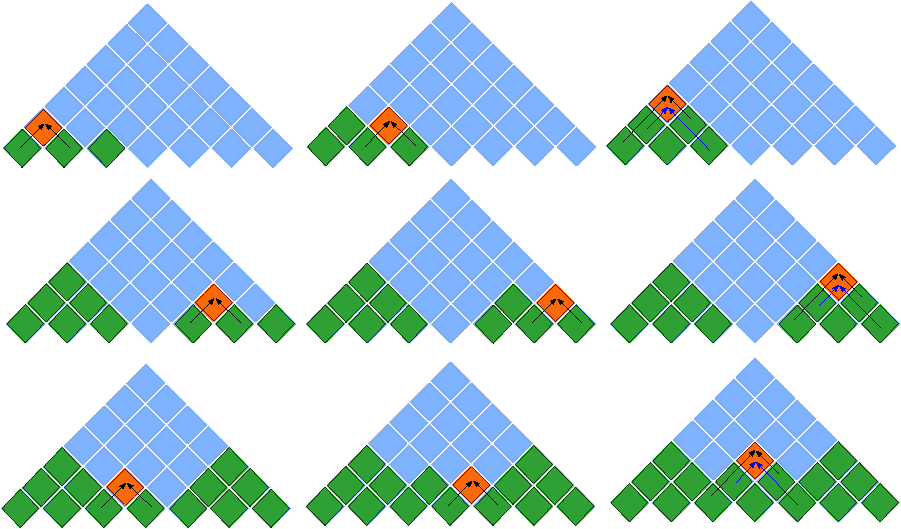
\includegraphics[width=0.600\textwidth]{pictures/valbeg.pdf}
    \caption{An example of beginning of Valiant's algorithm}
    \label{fig1}
\end{figure}

The procedure $compute(l, m)$ constructs the correct values of $T_{i,j} \forall l \le i < j < m$.

The procedure $complete(l, m, l', m')$ constructs the submatrix $\forall T_{i, j}$ $l \le i < m$, $l' \le j < m'$. This procedure assumes $T_{i, j} \forall l \leq i < j < m,  l' \leq i < j < m'$ are already constructed and the current value of  $P[i, j] =  \{ (B, C) |\exists (m \le k < l'): a_{i + 1} \dots a_{k} \in L(B), a_{k + 1} \dots a_{j} \in L(C)\}$ $\forall l \leq i < m,  l' \leq j < m'$. The submatrix division during the procedure call is shown in figure~\ref{fig2}.

Then Valiant described that product of multiplying of two submatrices of parsing table $T$ can be provided as $|N|^2$ Boolean matrices (for each pair of nonterminals). Denote matrix corresponding to pair $(B, C) \in N \times N$ as $Z^{(B, C)}$, then $Z_{i, j}^{(B, C)} = 1$ if and only if $(B, C) \in Z_{i, j}$. It should also be noted that $Z^{(B, C)} = X^{B} \times Y^{C}$. So, matrix multiplication in definition~\ref{def:defn4} can be replaced by Boolean matrix multiplication, each of which can be computed independently. Following these changes, time complexity of algorithm in listing~\ref{algo:valiant} is $O(|G|BMM(n)log(n))$ for an input string of length $n$, where $BMM(n)$ is the number of operations needed to multiply two Boolean matrices of size $n \times n$.

\begin{figure}
    \centering
    \captionsetup{justification=centering}
    \begin{minipage}{0.40\textwidth}
        \centering
        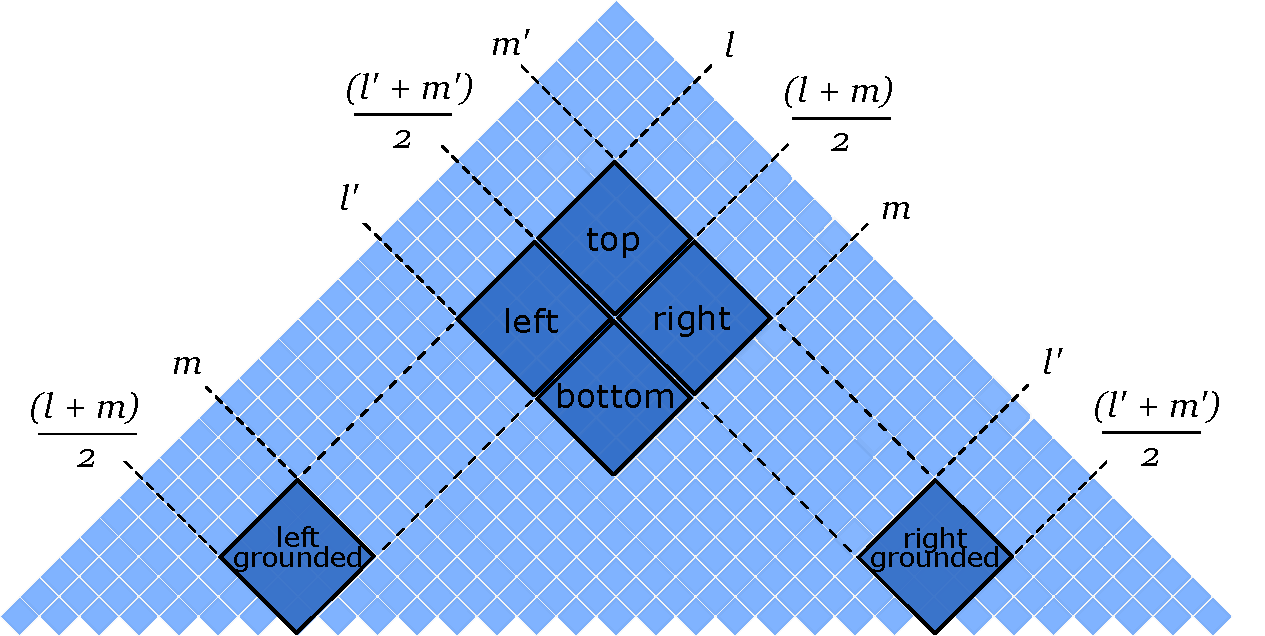
\includegraphics[width=1\textwidth]{pictures/splitting_with_grounded.pdf}
        \caption{Matrix partition used in \linebreak \textit{complete(l, m, l', m')} procedure.}
        \label{fig2}
    \end{minipage}\hfill
    \begin{minipage}{0.40\textwidth}
        \centering
        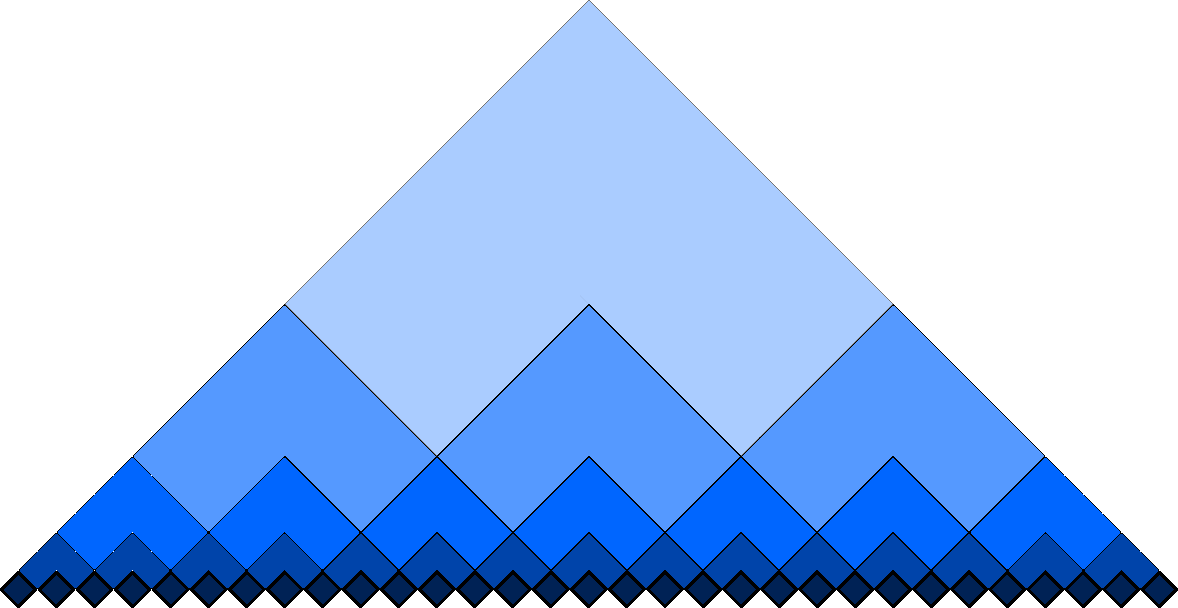
\includegraphics[width=1\textwidth]{pictures/layers.pdf}
        \caption{Matrix partition on V-shaped layers.}
        \label{fig3}
    \end{minipage}
\end{figure}

\section{Modified Valiant's algorithm}

In this section we describe the reorganization of submatrix processing order in the Valiant's algorithm which simplify independent handling of submatrices. As a result, proposed modification can facilitate implementation of parallel submatrix processing.

\subsection{New approach}

The main change of this modification is the possibility to divide the parsing table into layers of disjoint submatrices of the same size.
The idea of division we have made from the reorganization of the matrix multiplication order is presented in figure~\ref{fig3}.
Each layer consists of square matrices which size is power of 2.
The layers are computed successively in the bottom-up order.
Each matrix in the layer can be handled independently, which can help to implement parallel version of layer processing function.

\begin{figure}
    \centering
    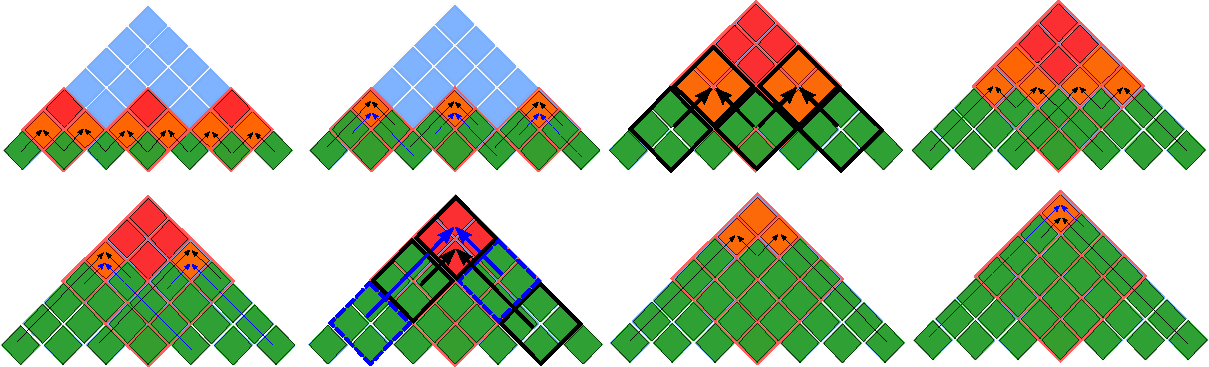
\includegraphics[width=0.9\textwidth]{pictures/modivis.pdf}
    \caption{An example of the modification of Valiant's algorithm}
    \label{fig4}
\end{figure}

A simple example of the modification process is shown in figure~\ref{fig4}. 
The lowest layer (submatrices which size is 1) is already computed and filling of the matrix starts with the second layer (????subfigures???? 1-2). 
Note that the same  process is presented in figure~\ref{fig1}, but here it can be done only in two steps using parallel computation of submatrix products.

The modified version of Valiant's algorithm is presented in listing~\ref{algo:modified}.
The procedure \textit{main()} computes the lowest layer $(T_{l, l+1})$, and then divide the table into layers, described earlier, and computes them through the \textit{completeVLayer()} call.
Thus, \textit{main()} computes all elements of parsing table $T$.
(Hereinafter, we use layer to mean set of submatrices.)

For brevity, we define \textit{left(subm), right(subm), top(subm), bottom(subm), rightgrounded(subm)} and \textit{leftgrounded(subm)} functions which returns the submatrices for matrix $subm = (l, m, l', m')$ according to the original Valiant's algorithm (figure~\ref{fig2}).

Also denote some subsidiary functions for matrix layer $M$:
 \begin{itemize}
  \item \textit{bottomsublayer(M)} $ = \{bottom(subm) | subm \in M \}$,
  \item \textit{leftsublayer(M)} $ = \{\textit{left(subm)} | subm \in M \}$,
  \item \textit{rightsublayer(M)} $ =\{\textit{right(subm)} | subm \in M \}$,
  \item \textit{topsublayer(M)} $ = \{top(subm) | subm \in M \}$.
\end{itemize}

\begin{algorithm}[h!]
\SetAlgoNoLine
\KwIn{$G = (\Sigma, N, R, S), w = a_{1} \dots a_{n}, n \geq 1, n + 1 = 2^p, a_{i} \in \Sigma$ }
\underline{main()}{:}{

 \For {$l \in \{1, \ldots, n \}$}{$T_{l, l + 1} = \{A | A \rightarrow a_{l + 1} \in R\}$}
 \For{$1 \le i < k $}{
 layer = \textit{constructLayer(i)}\;
 \textit{completeVLayer(layer)}
 }
 \BlankLine
 }

\underline{constructLayer(i)}{:}{
 \BlankLine
 $\{B | \exists k \geq 0 : B = (k*2^i, (k+1)*2^i, (k + 1)*2^i, (k+2)*2^i) \}$
 \BlankLine
    }
\underline{completeLayer(M)}{:}{
\BlankLine
\If {$\forall (l, m, l', m') \in M \quad (m - l = 1)$}{\For{$ (l, m, l', m') \in M$}{$T_{l, l'} = f(P_{l, l'})$\;}}
\Else{
\textit{completeLayer(bottomsublayer(M))}\;
\textit{completeVLayer(M)}
}
\BlankLine
}

\underline{comleteVLayer(M)}{:}{
 \BlankLine
 \textit{multiplicationTasks$_1$ = \{left$(m_i)$, leftgrounded$(m_i)$, bottom$(m_i) | m_i \in M \} \cup \linebreak  \{right(subm), bottom(subm), rightgrounded(subm) | subm \in M\}$\;}
 \BlankLine
 multiplicationTask$_2$ = $\{top(subm), leftgrounded(subm), right(subm) | subm \in M\}$\;
 \BlankLine
 multiplicationTask$_3$ = $\{top(subm), left(subm), rightgrounded |subm \in M\}$\;
 \BlankLine
 \textit{performMultiplications(multiplicationTask$_1$)}\;
 \textit{completeLayer(leftsublayer(M) $\cup$ rightsublayer(M))}\;
 \textit{performMultiplications(multiplicationTask$_2$)}\;
 \textit{performMultiplications(multiplicationTask$_3$)}\;
 \textit{completeLayer(topsublayer(M))}

 }
 \BlankLine

 \underline{performMultiplication(tasks)}{:}{\\
 \For{$ (m, m1, m2) \in \textit{tasks}$}{$P_{m} = P_{m} \cup (T_{m1} \times T_{m2})$\;}
 }

\caption{Parsing by matrix multiplication: Modified Version}
\label{algo:modified}
\end{algorithm}

The procedure \textit{completeVLayer(M)} takes an array of disjoint submatrices $M$ which represents a layer.
For each \textit{subm = (l, m, l', m') $\in M$} this procedure computes \textit{left(subm), right(subm), top(subm)}.
The procedure assumes that the elements of \textit{bottom(subm)} and $T_{i, j}$ for all $i$ and $j$ such that $l \leq i < j < m$ and $  l' \leq i < j < m'$ are already constructed.
Also it is assumed that the current value of
$P_{i, j} =  \{ (B, C) | \exists k, (m \le k < l'), a_{i + 1} \dots a_{k} \in L_G(B), a_{k + 1} \dots a_{j} \in L_G(C)\} $ for all $i$ and $j$ such that $l \leq i < m$ and $l' \leq j < m'$.

The procedure \textit{completeLayer(M)} also takes an array of disjoint submatrices $M$, but unlike the previous one, it computes $T_{i, j}$ for all $(i, j) \in subm$.
This procedure requires exactly same assumptions on $T_{i, j}$  and $P_{i, j}$  as in the previous case.

In the other words, \textit{completeVLayer(M)} computes the entire layer \textit{M} \linebreak and \textit{completeLayer($M_{2}$)} is a support function which is necessary for computation of smaller square submatrices $subm_{2} \in M_{2}$ inside of \textit{M}.  

Finally, the procedure \textit{performMultiplication(tasks)}, where \textit{tasks} is an array of a triple of submatrices, perform basic step of algorithm: matrix multiplication. It is worth mentioning that, as distinct from the original algorithm, here $|tasks| \ge 1$ and each task can be computed independently.
So, practical implementation of this procedure can easily involve different techniques of parallel array processing, such as OpenMP~\ref{!!!}.


\subsection{Correctness and complexity}

We provide the proof of correctness and time complexity for the proposed modification in this section.
To do it we should prove correctness of subprocedure \textit{completeLayer}.

\begin{theorem}
Let $M$ be a layer. If for all $(l, m, l', m') \in M$:
\begin{enumerate}
  \item $T_{i, j} = \{ A |  a_{i + 1} \dots a_{j} \in L_G(A)\}$ for all $i$ and $j$ such that $l \leq i < j < m$ and $l' \leq i < j < m'$;
  \item $P_{i, j} =  \{ (B, C) |\exists k, (m \le k < l'): a_{i + 1} \dots a_{k} \in L_G(B), a_{k + 1} \dots a_{j} \in L_G(C)\}$ for all $l \leq i < m$ and $l' \leq j < m'$.
\end{enumerate}

Then the procedure \textit{completeLayer(M)}, returns correctly computed sets of $T_{i, j}$ for all $l \leq i \le m$ and $l' \leq j \le m'$ for all $(l, m, l', m') \in M$.
\end{theorem}

\begin{comment}
\begin{proof}(Proof by induction on $m - l$.)

Let $(l, m, l', m')$ is a typical element of array $M$.
As far as each element can be handled independently, we prove statements only for one element of $M$.

\underline{\textbf{Basis:}} $m - l = 1$. There is only one element to compute, and $P_{l, l'} =  \{ (B, C) |  a_{l + 1} \dots a_{l'} \in L(B)L(C)\}$. Further, algorithm computes $f(P[l, l'])$ = \linebreak $\{ A |  a_{l + 1} \dots a_{l'} \in L(A)\}$, so $T[l, l']$ computed correctly.

\underline{\textbf{Inductive step:}} Assume that $(l_1, m_1, l_2, m_2)$ is correctly computed for $m_2 - l_2 = m_1 - l_1 > m - l$.

Let us consider complete \textit{completeLayer(M)}, where $m - l > 1$.

Firstly, consider \textit{completeLayer(bottom(M))}.
Theorem conditions are fulfilled, then this call returns correct sets $T_{i, j}$ for all $(i, j) \in bottom$ (hereinafter is means $\forall (i, j) \in m, \forall m \in \textit{bottom} $).
All submatrices with size $ m_1 - l_1 > m - l $, all previous layers and also \textit{bottom(M)} are correct, so,  \textit{completeVLayer(M)} can be called, and \textit{multiplicationByTask(task1)} adds to each
$ P[i, j] \forall (i, j) \in left(M) $
all pairs
$ \{(B, C) |\exists (\frac{l+m}{2} \le k < l'): a_{i + 1} \dots a_{k} \in L(B), a_{k + 1} \dots a_{j} \in L(C)\} $
 and
$ \forall (i, j) \in right (M)) $
 all pairs
$ \{ (B, C) |\exists (m \le k < \frac{l'+m'}{2}): a_{i + 1} \dots a_{k} \in L(B), a_{k + 1} \dots a_{j} \in L(C)\}$.
Now all the theorem conditions are fulfilled so, it is possible to call $\textit{completeLayer(left } \cup  \ right)$, which returns correct sets $T[i, j] \forall (i, j) \in (left \cup right)$.

Next, \textit{multiplicationByTask(task2)} and \textit{multiplicationByTask(task3)} add to each $P[i, j]$ $\forall (i, j) \in top = \{(l, \frac{l+m}{2}, \frac{l'+m'}{2}, m'))\}$ all pairs $\{(B, C) |\exists (\frac{l+m}{2} \le k < m)$ and $(l' \le k < \frac{l'+m'}{2}) : a_{i + 1} \dots a_{k} \in L(B), a_{k + 1} \dots a_{j} \in L(C)\}$. Now all the theorem conditions are fulfilled so, it is possible to call $\textit{completeLayer(top)}$, which returns correct sets $T[i, j]$ $\forall (i, j) \in top$.

Thus, all $T[i, j]$ $\forall (i, j) \in M$ are computed correctly.
\end{proof}
\end{comment}


\begin{theorem}
Algorithm from listing~\ref{algo:modified} correctly computes $T_{i, j}$ for all i and j, thus an input string $a = a_{1}a_{2} \dots a_{n} \in L_{G}(S)$ if and only if $S \in T_{0, n}$.
\end{theorem}

\begin{proof}

Primarily to prove the theorem, we show by induction that all layers of the parsing table T are computed correctly.

\underline{\textbf{Basis:}} layer of size $1 \times 1$.
Parsing table \textit{T} consists of one layer of size 1 and its elements are correctly computed in lines 2-3 in listing~\ref{algo:modified}.

\underline{\textbf{Inductive step:}} assume any layer of size less than or equal to $2^{p - 2} \times 2^{p - 2}$ are computed correctly. 

Define layer of size $2^{p - 1} \times 2^{p - 1}$ as M. 
Hereinafter \textit{subm = (l, m, l', m')} is a typical element of layer M.

Consider \textit{completeVLayer(M)} call. 

All $T_{i,j}$ are already calculated for all $i$ and $j$ such that $l \leq i < j < m$ and $l' \leq i < j < m'$, because these elements lie in layers which are already computed.

Firstly, \textit{performMultiplications(multiplicationTask$_1$)} adds to each P$_{i,j}$ all pairs 
$(B, C)$ such that $\exists k$, $(\frac{l+m}{2} \le k < l')$, $a_{i + 1} \dots a_{k} \in L_{G}(B)$, $a_{k + 1} \dots a_{j} \in L_{G}(C)$ for all $(i, j)$ $\in leftsublayer(M)$
and
$(B, C)$ such that $\exists k$, $(m \le k < \frac{l'+m'}{2})$, $a_{i + 1} \dots a_{k} \in L_{G}(B)$, $a_{k + 1} \dots a_{j} \in L_{G}(C)$ for all $(i, j)$ $\in rightsublayer(M)$.
Now \textit{completeLayer(leftsublayer(M) $\cup$ rightsublayer(M))} can be called and it returns correctly computed \textit{leftsublayer(M) $\cup$ rightsublayer(M)}.

Then \textit{performMultiplications} called with arguments 
\textit{multiplicationTask$_2$} and \textit{multiplicationTask$_3$} adds pairs 
$(B, C)$ such that $\exists k$, $(\frac{l+m}{2} \le k < m)$, $a_{i + 1} \dots a_{k} \in L_{G}(B)$, $a_{k + 1} \dots a_{j} \in L_{G}(C)$ 
and 
$(B, C)$ such that $\exists k$, $(l' \le k < \frac{l'+m'}{2})$, $a_{i + 1} \dots a_{k} \in L_{G}(B)$, $a_{k + 1} \dots a_{j} \in L_{G}(C)$
to each P$_{i,j}$ for all $(i, j)$ $\in topsublayer(M)$. 
So as $m = l'$ (from the construction of the layer), condition for elements of matrix $P$ are fulfilled.
Now \textit{completeLayer(topsublayer(M))} can be called and it returns correctly computed \textit{topsublayer(M)}.

Thus, \textit{completeVLayer(M)} returns correct $T_{i, j}$ for all $(i, j)$ $\in M$ for any layer M of parsing table T and lines 4-6 in listing~\ref{algo:modified} return all $T_{i, j} =  \{ A | A \in N, a_{i + 1} \dots a_{j} \in L_{G}(A)\}$.

\end{proof}

\begin{note}
Function $\textit{costructLayer(i)}$ returns $2^{k - i} - 1$ matrices of size $2^i$.
\end{note}

\begin{lemma}
\
\begin{itemize}
 \item $\forall i \in \{ 1, .., k - 1\}$  $\sum{|layer|}$ for the calls of \textit{completeVLayer(layer)} where $\forall (l, m, l', m') \in layer$ with $m - l = 2^{k - i}$  is exactly $2^{2i - 1} - 2^{i - 1}$;
 \item $\forall i \in \{ 1, .., k - 1\}$ products of submatrices of size $2^{k - i} \times 2^{k - i}$ are calculated exactly $2^{2i - 1} - 2^{i}$
\end{itemize}
\end{lemma}

\begin{proof}
The base case: i = 1. $\textit{completeVLayer(layer)}$ where $\forall (l, m, l', m') \in layer$ with $m - l = 2^{k - 1}$ is called only once in the  $\textit{main()}$ and $|layer| = 1$. So, $2^{2i - 1} - 2^{i - 1} = 2^1 - 2^0 = 1$.

For the induction step, assume that $\forall i \in \{ 1, .., j\}$ $\sum{|layer|}$ for the calls of $\textit{completeVLayer(layer)}$ where $\forall (l, m, l', m') \in layer$ with $m - l = 2^{k - i}$  which is exactly $2^{2i - 1} - 2^{i - 1}$.

Let us consider i = j + 1.

Firstly, it is the call of \textit{completeVLayer(costructLayer(k - i))}, where \textit{costructLayer(i)} returns $2^i - 1$ matrices of size $2^i$. Secondly, \textit{completeVLayer(layer)} is called 3 times for the left, right and top submatrices of size $2^{k - (i - 1)}$. Finally, \textit{completeVLayer(layer)} is called 4 times for the bottom, left, right and top submatrices of size $2^{k - (i - 2)}$, except $2^{i - 2} - 1$ matrices which were already computed.

Then, $\sum{|layer|} = 2^{i} - 1 + 3 \times (2^{2(i - 1) - 1} - 2^{(i - 1) - 1}) + 4 \times (2^{2(i - 2) - 1} - 2^{(i - 2) - 1}) - (2^{i - 2} - 1) = 2^{2i - 1} - 2^{i - 1}$.

To calculate the number of products of submatrices of size $2^{k - i} \times 2^{k - i}$, we consider the calls of \textit{completeVLayer(layer)} where $\forall (l, m, l', m') \in layer$ with $m - l = 2^{k - (i - 1)}$, which is $2^{2(i - 1) - 1} - 2^{(i - 1) - 1}$. During these calls \textit{performMultiplications} run 3 times, $|multiplicationTask1| = 2 \times 2^{2(i - 1) - 1} - 2^{(i - 1) - 1}$ and \linebreak $|multiplicationTask2|$ = $|multiplicationTask3| = 2^{2(i - 1) - 1} - 2^{(i - 1) - 1}$. So, the number of products of submatrices of size $2^{k - i} \times 2^{k - i}$ is $4 \times (2^{2(i - 1) - 1} - 2^{(i - 1) - 1}) = 2^{2i - 1} - 2^{i}$.
\end{proof}

\begin{theorem}
Let $|G|$ be a length of the description of the grammar G and let n be a length of an input string. Then algorithm from listing~\ref{algo:modified} calculates matrix \textit{T} in $\mathcal{O}(BMM(n)\log{n})$ where BMM(n) is the number of operations needed to multiply two Boolean matrices of size $n \times n$.
\end{theorem}

\begin{proof}
The proof is almost identical with that of the theorem given by Okhotin~\cite{Okhotin:2014:PMM:2565359.2565379}, because, as shown in the last lemma, the Algorithm 1 has the same number of products of submatrices.
\end{proof}

To summarize, the correctness of the modification was proved and it was shown that the time complexity remained the same as in Valiant's version.

\subsection{Algorithm for substrings}

Next we show how our modification can be applied to the string-matching problem.

So if we want to find all substrings of size $s$ which can be derived from a start symbol for an input string of size $n = 2^k$, we need to compute layers with submatrices of size not greater than $2^{l'}$, where $2^{l' - 2} < s \le 2^{l' - 1}$.

$l' = k - (m - 2)$, $(m - 2) = k - l'$

$ C \sum\limits_{i=m}^k 2^{2i - 1} \cdot 2^{\omega(k - i)} \cdot f(2^{k - i}) = C \cdot 2^{\omega l'}\sum\limits_{i=2}^{l'} 2^{(2 - \omega)i} \cdot 2^{2(k - l') - 1} \cdot f(2^{l' - i}) \le C \cdot 2^{\omega l'} f(2^{l'}) \cdot 2^{2(k - l') - 1} \sum\limits_{i=2}^{l'} 2^{(2 - \omega)i} = BMM(2^{l'}) \cdot 2^{2(k - l') - 1} \sum\limits_{i=2}^{l'} 2^{(2 - \omega)i}$

Thus, time complexity for searching all substrings is  $O(|G|BMM(2^{l'})(l' - 1))$, while time complexity for the full input string is $O(|G|BMM(2^k)(k - 1))$. In contract to the modification, Valiant's algorithm completely calculate at least 2 triangle submatrices of size $\frac{n}{2}$, which mean minimum asymptotic complexity  $O(|G|BMM(2^{k - 1})(k - 2))$. Make a conclusion that the modification is asymptotically faster for substrings of size $s \ll n$  than the original algorithm.

\begin{figure}
    \centering
    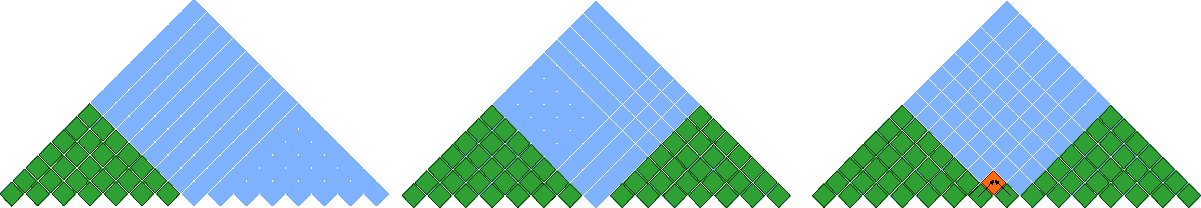
\includegraphics[width=0.9\textwidth]{pictures/valsubstring.pdf}
    \caption{first figure}
    \label{fig5}
\end{figure}

In order to test the resulting solution we have implemented the frontend as a plugin using ReSharper SDK, so it can be installed into ReSharper, Rider and InspectCode.
The source code is parsed by internal ReSharper tools and the result is used to produce graphs and meta-information.
The issues found by the backend are shown using code highlighting.

The first analysis which has been implemented is the considered taint tracking analysis.
It is defined just by the PDA constructed in the section 2 translated into the code with some slight modifications which make it possible to process interactions with object fields.
To provide more information about an issue found by this analysis, the higlighting is accompanied by bulbs containing the full path of tainted variable from the source to the sink represented as the sequence of operations.

\subsection{Sample cases}

Let's look closer at properties of the resulting soluiton.
All these properties are illustrated by screenshots taken exactly from the runned Rider IDE with some small relocations of bulbs to make them not to overlap the code.

Firstly, the solution ensures flow sensitivity. I.e. it processes flow of variables passed into methods and returned from them correctly.
Which can be seen at fig~\ref{fig:ReturnsAndBrackets}.
This example illustrates the most common cases of interprocedural data passing.
\textit{Brackets} method gets the data, performs some computations on them and returns the result.
Invocations at lines 37 and 38 shows that the solution can distinguish two data flow paths despite both of them passes through the same method.
So, \textit{e} becomes tainted because \textit{c} is tainted and \textit{f} does not because \textit{d} is clear.
Moreover, the solution can track paths where passes and returns do not form the correct bracket sequence that is shown by method \textit{PostSource} which does not take any parameter and just returns tainted data.

\begin{figure}[h]
	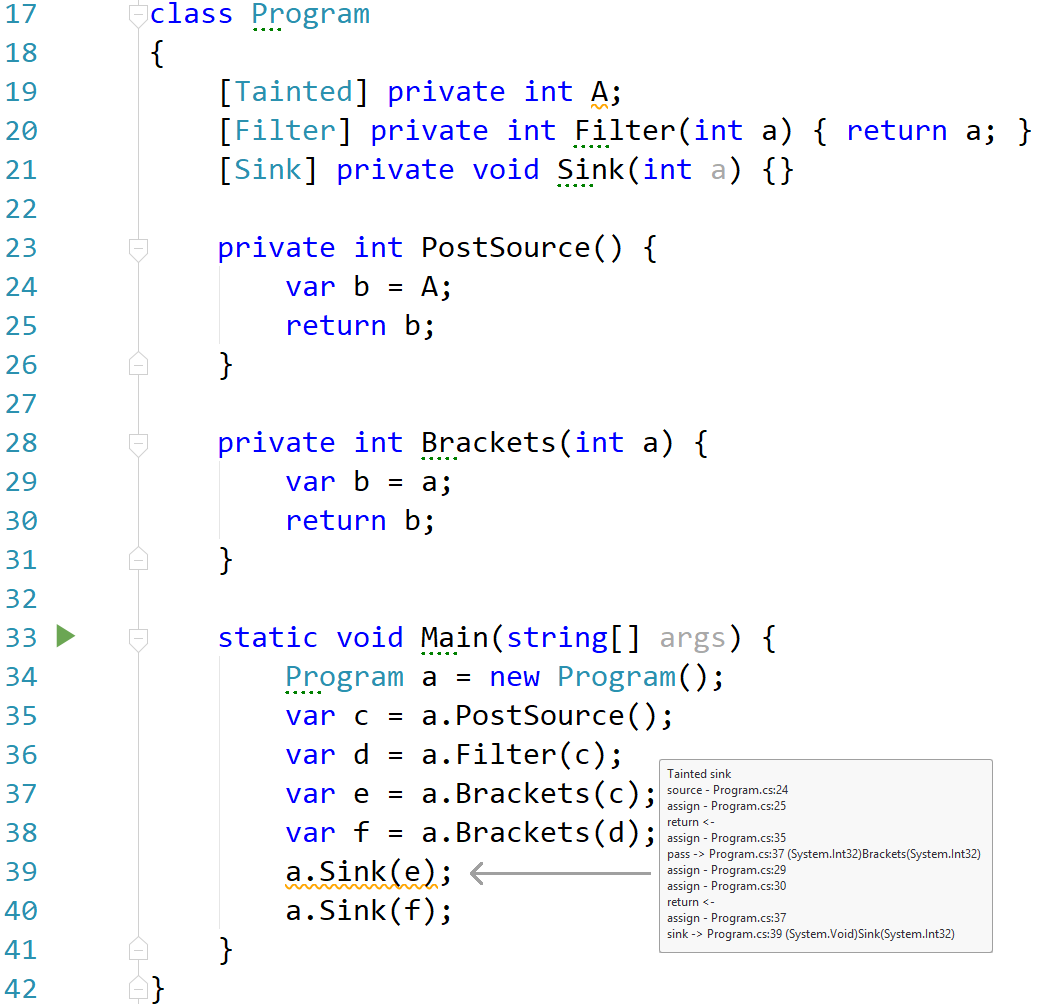
\includegraphics[width=\linewidth]{screenshots/ReturnsAndBrackets.png}
	\caption{Flow sensitivity}
	\label{fig:ReturnsAndBrackets}
\end{figure}

Secondly, the solution has the limited context sensitivity. I.e. it allows to track propagation of objects that are tainted by assigning of some fields inside them both by their own methods and by outer code interacting with their fields directly.
The first case is shown at fig~\ref{fig:ObjectTainting}.
There is the field \textit{B} at the line 18. 
This field can be used widely in the logic of the \textit{Container} class and by this the tainting of this field is considered as the tainting of the whole object.
However, while processing of the method \textit{Store} during the analysis it is hard to decide what the object need to be tainted because in the inner context of \textit{Store} it is just \textit{this} object.
I.e. we must consider the calling context to make such decision.
So, the solution provides this opportunity which is shown by lines 33-36 where the first invocation of \textit{Store} leads to the tainting of object \textit{d} and the second invocation does not taint object \textit{e}.

\begin{figure}[h]
	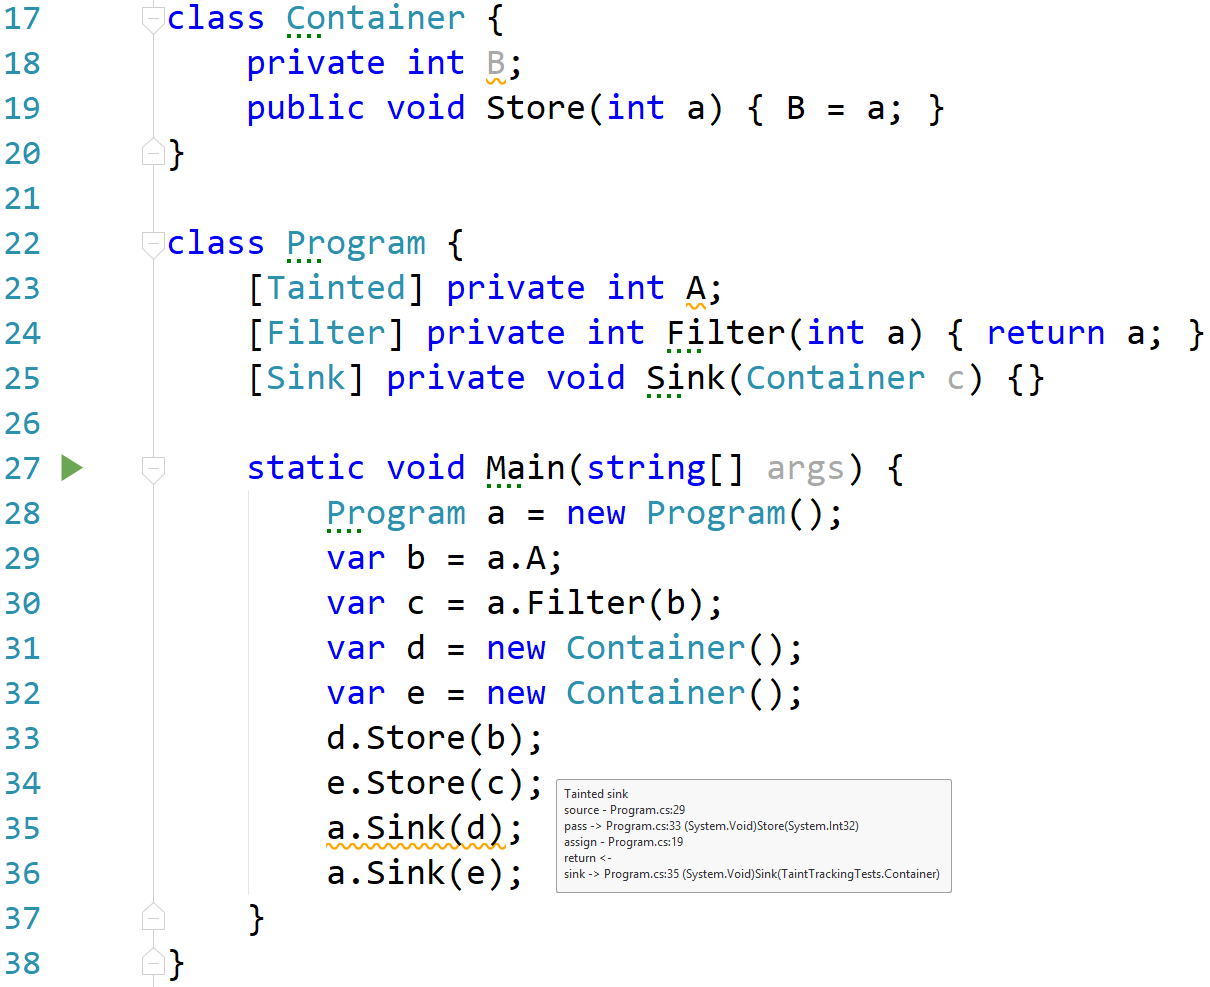
\includegraphics[width=\linewidth]{screenshots/ContextSensitivity.png}
	\caption{Tainting of an object by its own method}
	\label{fig:ObjectTainting}
\end{figure}

Finally, the solution works with any type of recursion and does not fall into infinite cycles.
It can be seen at fig.~\ref{fig:Recursion}.
This snippet contains two mutually recursive methods which pass the data to each other.
The solution checks all possible paths of passing even those which includes cyclic invocations and returns the passed variable to the point corresponding to the initial invocation.

\begin{figure}[h]
	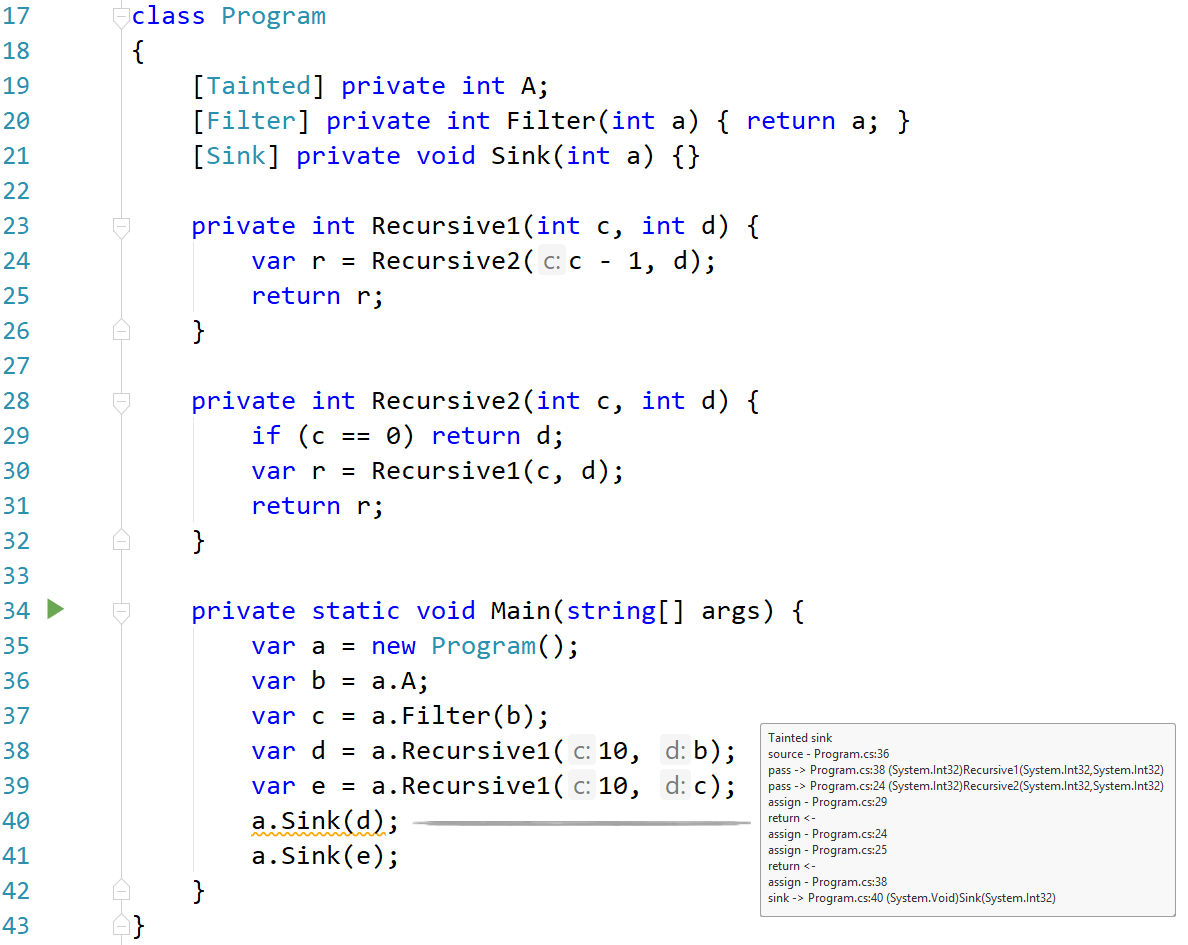
\includegraphics[width=\linewidth]{screenshots/Recursion.png}
	\caption{Recursive methods processing}
	\label{fig:Recursion}
\end{figure}

\subsection{Performance}

It is also necessary to measure the performance of the resulting solution.
Because the implemented taint tracking analysis forces to mark all participating entities manually, it is difficult to perform it on some large project.
However, there is another intermediate analysis which is runned before any other one to collect some information required by resolver.
In particular, it tracks propagation of all variables to discover all possible concrete types of each variable.
So, it involves each variable and each method in the whole program and thus the time and space required for execution of this analysis may be consistent estimation of the efficiency of the solution.

The code base that has been chosen as a source of data is the full solution of the Mono project.
(TODO: ADD SYSTEM CONFIGURATION).
The results is shown in the table~\ref{tab:Performance}.

\begin{table}[h]
	\begin{tabular}{|l|l|l|l|l|}
	\hline
		Project & Classes & Methods & \begin{tabular}[c]{@{}l@{}}Execution \\ time (s)\end{tabular} & \begin{tabular}[c]{@{}l@{}}Allocated \\ memory (GB)\end{tabular} \\ \hline
		Mono & 21013 & 192745 & $21\pm 0.5$ & $\sim 4.2$ \\ \hline
	\end{tabular}
	\caption{Performance}
	\label{tab:Performance}
\end{table}

\section{Conclusion}

We propose and implement in C\# programming language the generic framework for interprocedural static code analysis implementation.
This framework allows one to implement arbitrary interprocedural analysis in terms of CFL-reachability.
By using the proposed framework, we implement a plugin upon ReSharper infrastructure which provides simple taint analysis and demonstrate that our solution can handle important real-world cases.
Also we show that the proposed framework can be used for real-world solutions analysis.

One of the directions for future work is a creation of analysis and its evaluation on real-world projects.
By this way, we want to get information which helps to improve the usability of our framework: tune performance, improve API, etc.
Also we should improve documentation and create more examples of usage.

Another direction is a practical evaluation of automatic fix location prediction by using minimum cuts method~\cite{10.1007/978-3-319-63390-9_27}.

Also we want to compare the proposed approach with other generic CFL-reachability based approaches for interprocedural code analysis cretion. For example, fith generation-based approach~\cite{LPAR-21:Cauliflower_Solver_Generator_for}, which idea is similar to parser generators.



%
% ---- Bibliography ----
%
% BibTeX users should specify bibliography style 'splncs04'.
% References will then be sorted and formatted in the correct style.
%
% \bibliographystyle{splncs04}
% \bibliography{mybibliography}
%
\begin{thebibliography}{8}
\bibitem{chomsky1}
Chomsky, N.: On certain formal properties of grammars. Information and control \textbf{2}(2), 137--167 (1959)

\bibitem{chomsky2}
Chomsky, N. and Schützenberger M. P.: The algebraic theory of context-free languages. In: Studies in Logic and the Foundations of Mathematics vol. 35. pp. 118--161 Elsevier (1963)

\bibitem{rivas}
Rivas, E. and Eddy, S. R: The language of RNA: a formal grammar that includes pseudoknots. Bioinformatics \textbf{16}(4), 334–-340 (2000)

\bibitem{knudsen}
Knudsen, B. and Hein, J.: RNA secondary structure prediction using stochastic context-free grammars and evolutionary history. Bioinformatics (Oxford, England) \textbf{15}(6), 446–-454 (1999)

\bibitem{yuan}
Yuan, C. and Lei, J. and Cole, J. and Sun, Y.: Reconstructing 16S rRNA genes in metagenomic data. Bioinformatics \textbf{31}(12), i35–-i43 (2015)

\bibitem{dowell}
Dowell, R. D. and Eddy, S. R.: Evaluation of several lightweight stochastic context-free grammars for RNA secondary structure prediction. BMC bioinformatics \textbf{5}(1), 71 (2004)

\bibitem{bernardy}
Bernardy, J.P., Claessen K.: Efficient divide-and-conquer parsing of practical context-free languages. In: ACM SIGPLAN Notices, vol. 48. no. 9, pp. 111-122 ACM (2013)

\bibitem{kasami}
Kasami, T.: An efficient recognition and syntax-analysis algorithm for context-free languages. Coordinated Science Laboratory Report no. R-257 (1966)

\bibitem{younger}
Younger, D.H.: Recognition and parsing of context-free languages in time n3. Information and control \textbf{10}(2), 189--208 (1967)

\bibitem{earley}
Earley, J.: An efficient context-free parsing algorithm. Communications of the ACM \textbf{13}(2), 94--102 (1970)

\bibitem{valiant}
Valiant, L. G.: General context-free recognition in less than cubic time. Journal of computer and system sciences \textbf{10}(2), 308--315 (1975)

\bibitem{okhotin}
Okhotin, A.: Parsing by matrix multiplication generalized to Boolean grammars. Theoretical Computer Science \textbf{516}, 101--120 (2014)

\bibitem{m4ri}
The M4RI Library---Version 20121224, \url{http://m4ri.sagemath.org}. Last accessed 5
Jan 2019


\end{thebibliography}
\end{document}
